% Diapo des avancements

\begin{frame}[c]
  \frametitle{Avancements}
 
  \fbox{\tval{\large Pour le controle de la repetitivité des actions}} 
 
\pause
\begin{itemize}
  \item Prise en main de OCaml
  \item Début de compréhension du code de ph-exec
  \item Introduction d'un processus puit pour empécher les actions de se rejouer
\end{itemize}

\fbox{\tval{\large Pour l'analyse par sous graphe}} 
\begin{itemize}
 \item en cours...
\end{itemize}

\fbox{\tval{\large Pour l'introduction des priorités dans le PH}} 
\begin{itemize}
 \item réflexion en cours...
\end{itemize}


%\textcolor{couleurtheme}{$\Rightarrow$} \fbox{\tval{\large Analyse???}} \textcolor{couleurtheme}{$\Leftarrow$}

\end{frame}


% ici on va faire un petit test pour Sweave
\begin{frame}[c]

Voici un exemple simple:
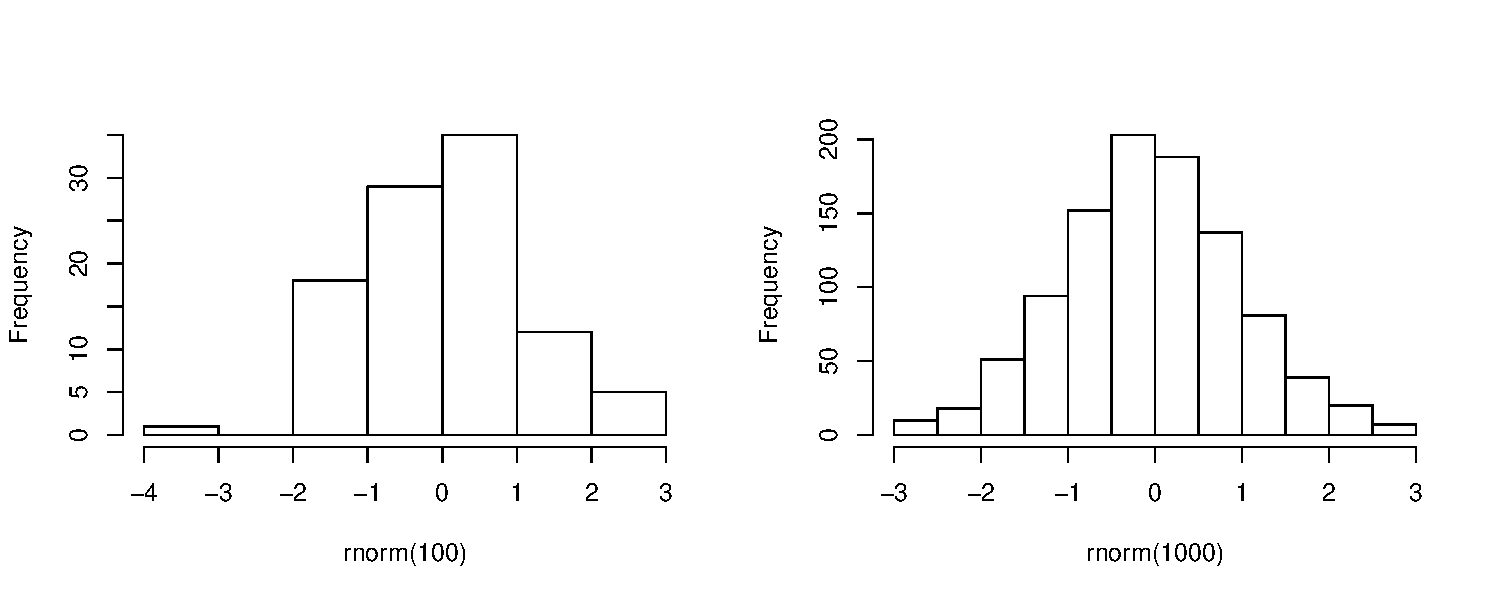
\includegraphics{avancement020414-exemple}

\end{frame}[c]

